\chapter{An Introduction to Groups}
\label{chapter:intro_groups}

%%----------------------------%%

One of the major topics of this course is \textbf{groups}.  The area of mathematics that is concerned with groups is called \textbf{group theory}. Loosely speaking, group theory is the study of symmetry, and in my opinion is one of the most beautiful areas in all of mathematics. It arises in puzzles, visual arts, music, nature, the physical and life sciences, computer science, cryptography, and of course, throughout mathematics.

%%----------------------------%%

\begin{section}{A First Example}\label{sec:first_example}

%%----------------------------%%

Let's begin our study by developing some intuition about what groups actually are.  To get started, we will explore the game Spinpossible\texttrademark, which used to be available for iOS and Android devices\footnote{If you'd like to play the game, try going here: \url{https://www.kongregate.com/games/spinpossible}.}.  The game is played on a $3\times 3$ board of scrambled tiles numbered 1 to 9, each of which may be right-side-up or up-side-down. The objective of the game is to return the board to the standard configuration where tiles are arranged in numerical order and right-side-up. This is accomplished by a sequence of ``spins", where a spin consists of rotating an $m\times n$ subrectangle by 180$^\circ$. The goal is to minimize the number of spins used.  The following figure depicts a scrambled board on the left and the solved board on the right.  The sequence of arrows is used to denote some sequence of spins that transforms the scrambled board into the solved board.

\begin{center}
\begin{tabular}{c}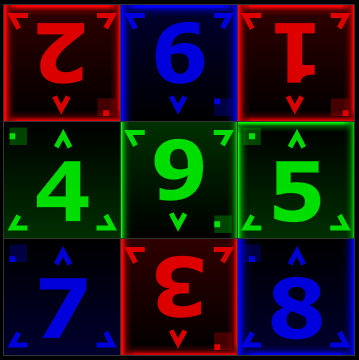
\includegraphics[width=1.5in]{scramble1.PNG}\end{tabular}
{\large $\xrightarrow{?} \cdots \xrightarrow{?}$}
\begin{tabular}{c}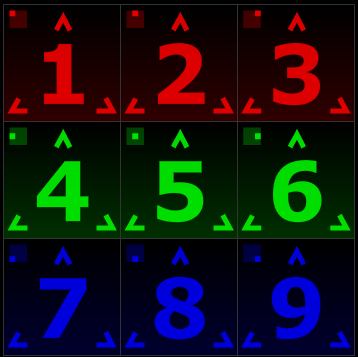
\includegraphics[width=1.5in]{scramble4.PNG}\end{tabular}
\end{center}

Let's play with an example.  Suppose we start with the following scrambled board.

\begin{center}
\begin{tikzpicture}[every node/.style={minimum size=.65cm}]
  \node [draw] (1) {\rotatebox{180}{$\underline{2}$}};
  \node [draw, right=0cm of 1] (2) {\rotatebox{180}{$\underline{9}$}};
  \node [draw, right=0cm of 2] (3) {\rotatebox{180}{$\underline{1}$}};
  \node [draw, below=0cm of 1] (4) {$\underline{4}$};
  \node [draw, right=0cm of 4] (5) {\rotatebox{180}{$\underline{6}$}};
  \node [draw, right=0cm of 5] (6) {$\underline{5}$};
  \node [draw, below=0cm of 4] (7) {$\underline{7}$};
  \node [draw, right=0cm of 7] (8) {\rotatebox{180}{$\underline{3}$}};
  \node [draw, right=0cm of 8] (9) {$\underline{8}$};
\end{tikzpicture}
\end{center}

\noindent The underlines on the numbers are meant to help us tell whether a tile is right-side-up or up-side-down.  Our goal is to use a sequence of spins to unscramble the board.  Before we get started, let's agree on some conventions.  When we refer to \emph{tile $n$}, we mean the actual tile that is labeled by the number $n$ regardless of its position and orientation on the board.  On the other hand, \emph{position $n$} will refer to the position on the board that tile $n$ is supposed to be in when the board has been unscrambled.  For example, in the board above, tile 1 is in position 3 and tile 7 happens to be in position 7.  

It turns out that there are multiple ways to unscramble this board, but I have one particular sequence in mind.  First, let's spin the rectangle determined by the two rightmost columns.  Here's what we get.  I've shaded the subrectangle that we are spinning.

\begin{center}
\begin{tabular}{c}
\begin{tikzpicture}[every node/.style={minimum size=.65cm}]
  \node [draw] (1) {\rotatebox{180}{$\underline{2}$}};
  \node [draw, fill=blue!40, right=0cm of 1] (2) {\rotatebox{180}{$\underline{9}$}};
  \node [draw, fill=blue!40, right=0cm of 2] (3) {\rotatebox{180}{$\underline{1}$}};
  \node [draw, below=0cm of 1] (4) {$\underline{4}$};
  \node [draw, fill=blue!40, right=0cm of 4] (5) {\rotatebox{180}{$\underline{6}$}};
  \node [draw, fill=blue!40, right=0cm of 5] (6) {$\underline{5}$};
  \node [draw, below=0cm of 4] (7) {$\underline{7}$};
  \node [draw, fill=blue!40, right=0cm of 7] (8) {\rotatebox{180}{$\underline{3}$}};
  \node [draw, fill=blue!40, right=0cm of 8] (9) {$\underline{8}$};
\end{tikzpicture}
\end{tabular}
%
{\large $\rightarrow$}
%
\begin{tabular}{c}
\begin{tikzpicture}[every node/.style={minimum size=.65cm}]
  \node [draw] (1) {\rotatebox{180}{$\underline{2}$}};
  \node [draw, right=0cm of 1] (2) {\rotatebox{180}{$\underline{8}$}};
  \node [draw, right=0cm of 2] (3) {$\underline{3}$};
  \node [draw, below=0cm of 1] (4) {$\underline{4}$};
  \node [draw, right=0cm of 4] (5) {\rotatebox{180}{$\underline{5}$}};
  \node [draw, right=0cm of 5] (6) {$\underline{6}$};
  \node [draw, below=0cm of 4] (7) {$\underline{7}$};
  \node [draw, right=0cm of 7] (8) {$\underline{1}$};
  \node [draw, right=0cm of 8] (9) {$\underline{9}$};
\end{tikzpicture}
\end{tabular}
\end{center}

\noindent Okay, now let's spin the middle column.

\begin{center}
\begin{tabular}{c}
\begin{tikzpicture}[every node/.style={minimum size=.65cm}]
  \node [draw] (1) {\rotatebox{180}{$\underline{2}$}};
  \node [draw, fill=blue!40, right=0cm of 1] (2) {\rotatebox{180}{$\underline{8}$}};
  \node [draw, right=0cm of 2] (3) {$\underline{3}$};
  \node [draw, below=0cm of 1] (4) {$\underline{4}$};
  \node [draw, fill=blue!40, right=0cm of 4] (5) {\rotatebox{180}{$\underline{5}$}};
  \node [draw, right=0cm of 5] (6) {$\underline{6}$};
  \node [draw, below=0cm of 4] (7) {$\underline{7}$};
  \node [draw, fill=blue!40, right=0cm of 7] (8) {$\underline{1}$};
  \node [draw, right=0cm of 8] (9) {$\underline{9}$};
\end{tikzpicture}
\end{tabular}
%
{\large $\rightarrow$}
%
\begin{tabular}{c}
\begin{tikzpicture}[every node/.style={minimum size=.65cm}]
  \node [draw] (1) {\rotatebox{180}{$\underline{2}$}};
  \node [draw, right=0cm of 1] (2) {\rotatebox{180}{$\underline{1}$}};
  \node [draw, right=0cm of 2] (3) {$\underline{3}$};
  \node [draw, below=0cm of 1] (4) {$\underline{4}$};
  \node [draw, right=0cm of 4] (5) {$\underline{5}$};
  \node [draw, right=0cm of 5] (6) {$\underline{6}$};
  \node [draw, below=0cm of 4] (7) {$\underline{7}$};
  \node [draw, right=0cm of 7] (8) {$\underline{8}$};
  \node [draw, right=0cm of 8] (9) {$\underline{9}$};
\end{tikzpicture}
\end{tabular}
\end{center}

\noindent Hopefully, you can see that we are really close to unscrambling the board.  All we need to do is spin the rectangle determined by the tiles in positions 1 and 2.

\begin{center}
\begin{tabular}{c}
\begin{tikzpicture}[every node/.style={minimum size=.65cm}]
  \node [draw, fill=blue!40] (1) {\rotatebox{180}{$\underline{2}$}};
  \node [draw, fill=blue!40, right=0cm of 1] (2) {\rotatebox{180}{$\underline{1}$}};
  \node [draw, right=0cm of 2] (3) {$\underline{3}$};
  \node [draw, below=0cm of 1] (4) {$\underline{4}$};
  \node [draw, right=0cm of 4] (5) {$\underline{5}$};
  \node [draw, right=0cm of 5] (6) {$\underline{6}$};
  \node [draw, below=0cm of 4] (7) {$\underline{7}$};
  \node [draw, right=0cm of 7] (8) {$\underline{8}$};
  \node [draw, right=0cm of 8] (9) {$\underline{9}$};
\end{tikzpicture}
\end{tabular}
%
{\large $\rightarrow$}
%
\begin{tabular}{c}
\begin{tikzpicture}[every node/.style={minimum size=.65cm}]
  \node [draw] (1) {$\underline{1}$};
  \node [draw, right=0cm of 1] (2) {$\underline{2}$};
  \node [draw, right=0cm of 2] (3) {$\underline{3}$};
  \node [draw, below=0cm of 1] (4) {$\underline{4}$};
  \node [draw, right=0cm of 4] (5) {$\underline{5}$};
  \node [draw, right=0cm of 5] (6) {$\underline{6}$};
  \node [draw, below=0cm of 4] (7) {$\underline{7}$};
  \node [draw, right=0cm of 7] (8) {$\underline{8}$};
  \node [draw, right=0cm of 8] (9) {$\underline{9}$};
\end{tikzpicture}
\end{tabular}
\end{center}

\noindent Putting all of our moves together, here is what we have.

\begin{center}
\begin{tabular}{c}
\begin{tikzpicture}[every node/.style={minimum size=.65cm}]
  \node [draw] (1) {\rotatebox{180}{$\underline{2}$}};
  \node [draw, fill=blue!40, right=0cm of 1] (2) {\rotatebox{180}{$\underline{9}$}};
  \node [draw, fill=blue!40, right=0cm of 2] (3) {\rotatebox{180}{$\underline{1}$}};
  \node [draw, below=0cm of 1] (4) {$\underline{4}$};
  \node [draw, fill=blue!40, right=0cm of 4] (5) {\rotatebox{180}{$\underline{6}$}};
  \node [draw, fill=blue!40, right=0cm of 5] (6) {$\underline{5}$};
  \node [draw, below=0cm of 4] (7) {$\underline{7}$};
  \node [draw, fill=blue!40, right=0cm of 7] (8) {\rotatebox{180}{$\underline{3}$}};
  \node [draw, fill=blue!40, right=0cm of 8] (9) {$\underline{8}$};
\end{tikzpicture}
\end{tabular}
%
{\large $\rightarrow$}
%
\begin{tabular}{c}
\begin{tikzpicture}[every node/.style={minimum size=.65cm}]
  \node [draw] (1) {\rotatebox{180}{$\underline{2}$}};
  \node [draw, fill=blue!40, right=0cm of 1] (2) {\rotatebox{180}{$\underline{8}$}};
  \node [draw, right=0cm of 2] (3) {$\underline{3}$};
  \node [draw, below=0cm of 1] (4) {$\underline{4}$};
  \node [draw, fill=blue!40, right=0cm of 4] (5) {\rotatebox{180}{$\underline{5}$}};
  \node [draw, right=0cm of 5] (6) {$\underline{6}$};
  \node [draw, below=0cm of 4] (7) {$\underline{7}$};
  \node [draw, fill=blue!40, right=0cm of 7] (8) {$\underline{1}$};
  \node [draw, right=0cm of 8] (9) {$\underline{9}$};
\end{tikzpicture}
\end{tabular}
%
{\large $\rightarrow$}
%
\begin{tabular}{c}
\begin{tikzpicture}[every node/.style={minimum size=.65cm}]
  \node [draw, fill=blue!40] (1) {\rotatebox{180}{$\underline{2}$}};
  \node [draw, fill=blue!40, right=0cm of 1] (2) {\rotatebox{180}{$\underline{1}$}};
  \node [draw, right=0cm of 2] (3) {$\underline{3}$};
  \node [draw, below=0cm of 1] (4) {$\underline{4}$};
  \node [draw, right=0cm of 4] (5) {$\underline{5}$};
  \node [draw, right=0cm of 5] (6) {$\underline{6}$};
  \node [draw, below=0cm of 4] (7) {$\underline{7}$};
  \node [draw, right=0cm of 7] (8) {$\underline{8}$};
  \node [draw, right=0cm of 8] (9) {$\underline{9}$};
\end{tikzpicture}
\end{tabular}
%
{\large $\rightarrow$}
%
\begin{tabular}{c}
\begin{tikzpicture}[every node/.style={minimum size=.65cm}]
  \node [draw] (1) {$\underline{1}$};
  \node [draw, right=0cm of 1] (2) {$\underline{2}$};
  \node [draw, right=0cm of 2] (3) {$\underline{3}$};
  \node [draw, below=0cm of 1] (4) {$\underline{4}$};
  \node [draw, right=0cm of 4] (5) {$\underline{5}$};
  \node [draw, right=0cm of 5] (6) {$\underline{6}$};
  \node [draw, below=0cm of 4] (7) {$\underline{7}$};
  \node [draw, right=0cm of 7] (8) {$\underline{8}$};
  \node [draw, right=0cm of 8] (9) {$\underline{9}$};
\end{tikzpicture}
\end{tabular}
\end{center}
In this case, we were able to solve the scrambled board in 3 moves.  It's not immediately obvious, but it turns out that there is no way to unscramble the board in fewer than 3 spins.  However, there is at least one other solution that involves exactly 3 spins.

\begin{problem}\label{prob:number_spinpossible_boards}
How many scrambled $3\times 3$ Spinpossible boards are there?  To answer this question, you will need to rely on some counting principles such as factorials. In this context, we want to include the solved board as one of the scrambled boards---it's just not very scrambled.
\end{problem}

\begin{problem}\label{prob:counting_spins}
How many spins are there?
\end{problem}

It's useful to have some notation. Let $s_{ij}$ denote the spin that rotates the subrectangle that has position $i$ in the upper-left corner and position $j$ in the lower-right corner.  As an example, the sequence of spins that we used above to unscramble our initial scrambled board is
\[
s_{29}\to s_{28} \to s_{12}.
\]
As you noticed in Problem~\ref{prob:counting_spins}, we can also rotate a single tile. Every spin of the form $s_{ii}$ is called a \emph{toggle}. For example, $s_{44}$ toggles the tile in position 4. 

We can think of each spin as a function and since we are doing spins on top of spins, every sequence of spins corresponds to a composition of functions. We will follow the standard convention of function composition that says the function on the right goes first.  In this case, our previous sequence of spins becomes $s_{12} \circ s_{28}  \circ s_{29}$, which we abbreviate as $s_{12} s_{28} s_{29}$. This might take some getting used to, but just remember that it is just like function notation---stuff on the right goes first. We will refer to expressions like $s_{12} s_{28} s_{29}$ as \textbf{words} in the alphabet $\{s_{ij}\mid i\text{ upper left corner}, j\text{ lower right corner of subrectangle}\}$.  Our words will always consist of a finite number of spins.

Every word consisting of spins corresponds to a function that takes a scrambled board as input and returns a scrambled board. We say that the words ``act on" the scrambled boards. For each word, there is an associated \textbf{net action}. For example, the word $s_{12} s_{23} s_{12}$ corresponds to swapping the positions but not orientation of the tiles in positions 1 and 3.  You should take the time to verify this for yourself. Notice that the net action does not depend on the current configuration of the board. Sometimes it is difficult to describe what the net action associated to a word is, but there is always some corresponding net action nonetheless. Moreover, each net action has many---infinitely many, in fact---words that determine that net action. For example, it turns out that $s_{12}s_{23}s_{12}$, $s_{23}s_{12}s_{23}$, and $s_{12}s_{23}s_{11}s_{11}s_{12}$ all yield the same net action.   In this case, we would write
\[
s_{12}s_{23}s_{12}=s_{23}s_{12}s_{23}=s_{12}s_{23}s_{11}s_{11}s_{12}.
\]
Notice that equality here is referring to net action and not the words themselves.  That is, the words are different, but the result is the same.

It is worth pointing out that $s_{12} s_{23} s_{12}$ is not itself a spin.  However, sometimes a composition of spins will yield a spin.  For example, the net action of $s_{12} s_{11} s_{12}$ is toggling the tile in position 2.  That is, $s_{12} s_{11} s_{12}=s_{22}$.

\begin{problem}\label{prob:3_different_spins}
Find a sequence of 3 spins that is different from the one we described earlier that unscrambles the following board. Write your answer as a word consisting of spins.
\begin{center}
\begin{tikzpicture}[every node/.style={minimum size=.65cm}]
  \node [draw] (1) {\rotatebox{180}{$\underline{2}$}};
  \node [draw, right=0cm of 1] (2) {\rotatebox{180}{$\underline{9}$}};
  \node [draw, right=0cm of 2] (3) {\rotatebox{180}{$\underline{1}$}};
  \node [draw, below=0cm of 1] (4) {$\underline{4}$};
  \node [draw, right=0cm of 4] (5) {\rotatebox{180}{$\underline{6}$}};
  \node [draw, right=0cm of 5] (6) {$\underline{5}$};
  \node [draw, below=0cm of 4] (7) {$\underline{7}$};
  \node [draw, right=0cm of 7] (8) {\rotatebox{180}{$\underline{3}$}};
  \node [draw, right=0cm of 8] (9) {$\underline{8}$};
\end{tikzpicture}
\end{center}
\end{problem}

\begin{problem}
What is the net action that corresponds to the word $s_{23} s_{12} s_{23}$? What can you conclude about $s_{23} s_{12} s_{23}$ compared to 
$s_{12} s_{23} s_{12}$?
\end{problem}

We can also use exponents to abbreviate.  For example, $s_{23}^2$ is the same as $s_{23} s_{23}$ (which in this case is the net action of doing nothing) and $(s_{12} s_{23})^2$ is the same as $s_{12} s_{23} s_{12} s_{23}$.

\begin{problem}\label{prob:braid_relation}
It turns out that there is an even simpler word (i.e., a shorter word) that yields the same net action as $(s_{12} s_{23})^2$. Can you find one?
\end{problem}

Define $\Spin_{3\times 3}$ to be the collection of net actions that we can obtain from words consisting of spins.  We say that the set of spins \textbf{generates} $\Spin_{3\times 3}$ and we refer to the set of spins as a \textbf{generating set} for $\Spin_{3\times 3}$.  

\begin{problem}
Suppose $s_{x_1}s_{x_2}\cdots s_{x_n}$ and $s_{y_1}s_{y_2}\cdots s_{y_m}$ are both words consisting of spins. Then the corresponding net actions, say $u$ and $v$, respectively, are elements of $\Spin_{3\times 3}$. Prove that the composition of the actions $u$ and $v$ is an element of $\Spin_{3\times 3}$.
\end{problem}

The previous problem tells us that the composition of two net actions from $\Spin_{3\times 3}$ results in another net action in $\Spin_{3\times 3}$. Formally, we say that $\Spin_{3\times 3}$ is \textbf{closed} under composition.

It is clear that we can construct an infinite number of words consisting of spins, but since there are a finite number of ways to rearrange the positions and orientations of the tiles of the $3\times 3$ board, there are only a finite number of net actions arising from these words.  That is, $\Spin_{3\times 3}$ is a finite set of functions.

\begin{problem}
Verify that $\Spin_{3\times 3}$ contains an \textbf{identity} function, i.e., a function whose net action is ``do nothing." What happens if we compose a net action from $\Spin_{3\times 3}$ with the identity?
\end{problem}

A natural question to ask is whether every possible scrambled Spinpossible board can be unscrambled using only spins.  In other words, is $\Spin_{3\times 3}$ sufficient to unscramble every scrambled board? It turns out that the answer is yes.

\begin{problem}\label{prob:kindergarten_algorthim}
Verify that $\Spin_{3\times 3}$ is sufficient to unscramble every scrambled board by describing an algorithm that will always unscramble a scrambled board.  It does not matter whether your algorithm is efficient.  That is, we don't care how many steps it takes to unscramble the board as long as it works in a finite number of steps.  Using your algorithm, what is the maximum number of spins required to unscramble any scrambled board?
\end{problem}

In a 2011 paper, Alex Sutherland and Andrew Sutherland (a father and son team) present a number of interesting results about Spinpossible and list a few open problems. You can find the paper at \url{http://arxiv.org/abs/1110.6645}. As a side note, Alex is one of the developers of the game and his father, Andrew, is a mathematics professor at MIT. Using a brute-force computer algorithm, the Sutherlands verified that every scrambled $3\times 3$ Spinpossible board can be solved in at most 9 moves. However, a human readable mathematical proof of this fact remains elusive.  By the way, mathematics is chock full of open problems and you can often get to the frontier of what is currently known without too much trouble.  Mathematicians are in the business of solving open problems.

Instead of unscrambling boards, we can act on the solved board with an action from $\Spin_{3\times 3}$ to obtain a scrambled board.  Problem~\ref{prob:kindergarten_algorthim} tells us that we can use $\Spin_{3\times 3}$ to get from the solved board to any scrambled board. In fact, starting with the solved board makes it clear that there is a one-to-one correspondence between net actions and scrambled boards.

\begin{problem}
What is the size of $\Spin_{3\times 3}$? That is, how many net actions are in $\Spin_{3\times 3}$?
\end{problem}

Let's make a couple more observations.  First, every spin is reversible. That is, every spin has an \textbf{inverse}.  In the case of Spinpossible, we can just apply the same spin again to undo it.  For example, $s_{12}^2$ is the same as doing nothing. This means that the inverse of $s_{12}$, denoted $s_{12}^{-1}$, is $s_{12}$ itself. Symbolically, we write $s_{12}^{-1}=s_{12}$. Remember that we are exploring the game Spinpossible---it won't always be the case that repeating an action will reverse the action. 

In the same vein, every sequence of spins is reversible. For example, if we apply $s_{12} s_{23}$ (i.e., do $s_{23}$ first followed by $s_{12}$), we could undo the net action by applying $s_{23} s_{12}$ because
\[
(s_{12} s_{23})^{-1}=s_{23}^{-1} s_{12}^{-1}=s_{23} s_{12}
\]
since $s_{23}^{-1}=s_{23}$ and $s_{12}^{-1}=s_{12}$.  Notice that the first equality is an instantiation of the ``socks and shoes theorem", which states that if $f$ and $g$ are functions with compatible domain and codomain, then
\[
(f\circ g)^{-1} = g^{-1}\circ f^{-1}.
\]
The upshot is that the net action that corresponds to a word consisting of spins can be reversed by applying ``socks and shoes" and is itself an action.

\begin{problem}
Imagine we started with the solved board and then you scrambled the board according to some word consisting of spins.  Let's call this word $w$. How could you obtain the solved board from the scrambled board determined by $w$? How is this related to $w^{-1}$?
\end{problem}

There is one detail we have been sweeping under the rug.  Notice that every time we wrote down a word consisting of two or more spins, we didn't bother to group pairs of adjacent spins using parentheses.  Recall that the composition of functions with compatible domains and codomains is \textbf{associative} (see Theorem~\ref{thm:function_comp_associative}).  That is, if $f$, $g$, and $h$ are functions with compatible domains and codomains, then
\[
(f\circ g)\circ h = f\circ (g\circ h).
\]
Since composition of spins is really just function composition, composition of spins is also associative.  And since the spins generate $\Spin_{3\times 3}$, the composition of net actions from $\Spin_{3\times 3}$ is associative, as well.

\begin{problem}
Does the order in which you apply spins matter?  Does it always matter?  Let's be as specific as possible.  If the order in which we apply two spins does not matter, then we say that the spins \textbf{commute}.  However, if the order does matter, then the spins do not commute.  When will two spins commute?  When will they not commute?  Provide some specific examples.
\end{problem}

In the previous problem, you discovered that the composition of two spins may or may not commute.  Since the spins generate $\Spin_{3\times 3}$, the composition of two net actions may or may not commute.  We say that $\Spin_{3\times 3}$ is not commutative.

Let's collect our key observations about $\Spin_{3\times 3}$.
\begin{enumerate}[label=\rm{(\arabic*)}]
\item \textbf{Generating Set:} The set of spins generates $\Spin_{3\times 3}$.  That is, every net action from $\Spin_{3\times 3}$ corresponds to a word consisting of spins.\footnote{The case of Spinpossible is a little misleading. Since each spin is its own inverse, we never need to write words consisting of spins with inverses. However, as we shall see later, there are situations outside the context of Spinpossible where we will need to utilize inverses of elements from a generating set.} 
\item \textbf{Closure:} The composition of any two net actions from $\Spin_{3\times 3}$ results in a net action from $\Spin_{3\times 3}$.
\item \textbf{Associative:} The composition of net actions from $\Spin_{3\times 3}$ is associative.
\item \textbf{Identity:} There is an identity in $\Spin_{3\times 3}$ whose corresponding net action is ``do nothing".
\item \textbf{Inverses:} Every net action from $\Spin_{3\times 3}$ has an inverse net action in $\Spin_{3\times 3}$. Composing a net action and its inverse results in the identity.
\item The composition of two net actions from $\Spin_{3\times 3}$ may or may not commute.
\end{enumerate}

It turns out that $\Spin_{3\times 3}$ is an example of a group. Loosely speaking, a \textbf{group} is a set together with a method for combining two elements together that satisfies conditions (2), (3), (4), and (5) above.  More formally, a group is a nonempty set together with an associative binary operation such that the set contains an identity element and every element in the set has an inverse that is also in the set.  As we shall see, groups can have a variety of generating sets, possibly of different sizes. Also, some groups are commutative and some groups are not.

Before closing out this section, let's tackle a few more interesting problems concerning Spinpossible. We say that a generating set $S$ for a group is a \textbf{minimal generating set} if $S\setminus\{x\}$ is no longer a generating set for the group for all $x\in S$.

\begin{problem}
Determine whether the set of spins is a minimal generating set for $\Spin_{3\times 3}$.
\end{problem}

It's not too difficult to prove---but we will omit the details---that we can generate $\Spin_{3\times 3}$ with the following subset of 9 spins:
\[
T=\{s_{11}, s_{12}, s_{23}, s_{36}, s_{56}, s_{45}, s_{47}, s_{78}, s_{89}\}.
\]
That is, every net action in $\Spin_{3\times 3}$ corresponds to a word consisting of the spins from $T$.  Try to take a moment to convince yourself that this is at least plausible.  

\begin{problem}
For each of the following spins, find a word consisting of spins from the set $T$ that yields the same net action.
\begin{enumerate}[label=\rm{(\alph*)}]
\item $s_{33}$
\item $s_{13}$
\item $s_{14}$
\end{enumerate}
\end{problem}

\begin{problem}
Taking for granted that $T$ is a generating set for $\Spin_{3\times 3}$, determine whether $T$ is a minimal generating set.
\end{problem}

\end{section}

%%----------------------------%%

\begin{section}{Binary Operations}

%%----------------------------%%

Before beginning our formal study of groups, we need to have an understanding of binary operations. After learning to count as a child, you likely learned how to add, subtract, multiply, and divide with real numbers.  As long as we avoid division by zero, these operations are examples of binary operations since we are combining two objects to obtain a single object.  More formally, we have the following definition.

\begin{definition}
A \textbf{binary operation} $*$ on a set $A$ is a function from $A\times A$ into $A$.  For each $(a,b)\in A\times A$, we denote the element $*(a,b)$ via $a*b$.  If the context is clear, we may abbreviate $a*b$ as $ab$.
\end{definition}

Don't misunderstand the use of $*$ in this context.  We are not implying that $*$ is the ordinary multiplication of real numbers that you are familiar with.  We use $*$ to represent a generic binary operation.  

Notice that since the codomain of a binary operation on a set $A$ is $A$, binary operations require that we yield an element of $A$ when combining two elements of $A$.  In this case, we say that $A$ is \textbf{closed} under $*$.  Binary operations have this closure property by definition.  Also, since binary operations are functions, any attempt to combine two elements from $A$ should result in a \emph{unique} element of $A$.  Moreover, since the domain of $*$ is $A\times A$, it must be the case that $*$ is defined for \emph{all} pairs of elements from $A$.

\begin{example}
Here are some examples of binary operations.
\begin{enumerate}[label=\rm{(\alph*)}]
\item The operations of $+$ (addition), $-$ (subtraction), and $\cdot$ (multiplication) are binary operations on the real numbers.  All three are also binary operations on the integers.  However, while $+$ and $\cdot$ are both binary operations on the set of natural numbers, $-$ is not a binary operation on the natural numbers since $1-2=-1$, which is not a natural number.
\item The operation of $\div$ (division) is not a binary operation on the set of real numbers because all elements of the form $(a,0)$ are not in the domain $\mathbb{R}\times \mathbb{R}$ since we cannot divide by 0.  Yet, $\div$ is a suitable binary operation on $\mathbb{R}\setminus \{0\}$.
\item Let $A$ be a nonempty set and let $F$ be the set of functions from $A$ to $A$.  Then $\circ$ (function composition) is a binary operation on $F$. We utilized this fact when exploring the game Spinpossible.
\item Let $M_{2\times 2}(\mathbb{R})$ be the set of $2\times 2$ matrices with real number entries.  Then matrix multiplication is a binary operation on $M_{2\times 2}(\mathbb{R})$.
\end{enumerate}
\end{example}

\begin{problem}
Let $M(\mathbb{R})$ be the set of matrices (of any size) with real number entries.  Is matrix addition a binary operation on $M(\mathbb{R})$?  How about matrix multiplication? What if you restrict to square matrices of a fixed size $n\times n$?
\end{problem}

\begin{problem}
Let $A$ be a set. Determine whether $\cup$ (union) and $\cap$ (intersection) are binary operations on $\mathcal{P}(A)$ (i.e., the power set of $A$).
\end{problem}

\begin{problem}
Consider the closed interval $[0,1]$ and define $*$ on $[0,1]$ via $a*b=\min(a,b)$ (i.e., take the minimum of $a$ and $b$).  Determine whether $*$ is a binary operation on $[0,1]$.
\end{problem}

\begin{problem}\label{prob:introducing_R4}
Consider a square puzzle piece that fits perfectly into a square hole.  Let $R_4$ be the set of net actions consisting of the rotations of the square by an appropriate amount so that it fits back into the hole. Assume we can tell the corners of the square apart from each other so that if the square has been rotated and put back in the hole we can notice the difference. Each net action is called a \textbf{symmetry} of the square. 
\begin{enumerate}[label=\rm{(\alph*)}]
\item Describe all of the distinct symmetries in $R_4$. How many distinct symmetries are in $R_4$?
\item Is composition of symmetries a binary operation on $R_4$?
\end{enumerate}
\end{problem}

Let's pause for a moment to make sure we understand our use of the word symmetry in this context. A fundamental question in mathematics is ``When are two things the same?", where ``things" can be whatever mathematical notion we happen to be thinking about at a particular moment. Right now we need to answer, ``When do we want to consider two symmetries to be the same?" To be clear, this is a choice, and different choices can lead to different, interesting, and equally valid mathematics. For symmetries, one natural thought is that symmetries are equal when they produce the same net action on the square, meaning that when applied to a square in a particular starting position, they both yield the same ending position. In general, two symmetries are equal if they produce the same net action on the object in question.

The set $R_4$ is called the rotation group for the square. For $n\geq 3$, $R_n$ is the \textbf{rotation group} for the regular $n$-gon and consists of the rotational symmetries for a regular $n$-gon. As we shall see later, every $R_n$ really is a group under composition of symmetries.

\begin{problem}\label{prob:introducing_D3}
Consider a puzzle piece like the one in the previous problem, except this time, let's assume that the piece and the hole are an equilateral triangle.  Let $D_3$ be the full set of symmetries that allow the triangle to fit back in the hole.  In addition to rotations, we will also allow the triangle to be flipped over---called a reflection. 
\begin{enumerate}[label=\rm{(\alph*)}]
\item Describe all of the distinct symmetries in $D_3$. How many distinct symmetries are in $D_3$?
\item Is composition of symmetries a binary operation on $D_3$?
\end{enumerate}
\end{problem}

\begin{problem}\label{prob:introducing_D4}
Repeat the above problem, but do it for a square instead of a triangle.  The corresponding set is called $D_4$.
\end{problem}

The sets $D_3$ and $D_4$ are examples of dihedral groups. In general, for $n\geq 3$, $D_n$ consists of the symmetries (rotations and reflections) of a regular $n$-gon and is called the \textbf{dihedral group of order $2n$}. In this case, the word ``order" simply means the number of symmetries in the set. Do you see why $D_n$ consists of $2n$ actions? As expected, we will prove that every $D_n$ really is a group.

\begin{problem}\label{prob:introducing_S3}
Consider the set $S_3$ consisting of the net actions that permute the positions of three coins (without flipping them over) that are sitting side by side in a line.  Assume that you can tell the coins apart.
\begin{enumerate}[label=\rm{(\alph*)}]
\item Write down all distinct net actions in $S_3$ using verbal descriptions. Some of these will be tricky to describe. How many distinct net actions are in $S_3$?
\item Is composition of net actions a binary operation on $S_3$?
\end{enumerate}
\end{problem}

The set $S_3$ is an example of a symmetric group. In general, $S_n$ is the \textbf{symmetric group on $n$ objects} and consists of the net actions that rearrange the $n$ objects. Such rearrangements are called \textbf{permutations}. Later we will prove that each $S_n$ is a group under composition of permutations.

\begin{problem}
Explain why composition of spins is not a binary operation on the set of spins in $\Spin_{3\times 3}$.
\end{problem}

Some binary operations have additional properties.

\begin{definition}
Let $A$ be a nonempty set and let $*$ be a binary operation on $A$.
\begin{enumerate}[label=\rm{(\alph*)}]
\item We say that $*$ is \textbf{associative} if and only if $(a*b)*c=a*(b*c)$ for all $a,b,c\in A$.
\item We say that $*$ is \textbf{commutative} if and only if $a*b=b*a$ for all $a,b\in A$.
\end{enumerate}
\end{definition}

\begin{problem}
Provide an example of each of the following.
\begin{enumerate}[label=\rm{(\alph*)}]
\item A binary operation on a set that is commutative.
\item A binary operation on a set that is not commutative.
\end{enumerate}
\end{problem}

\begin{problem}
Provide an example of a set $A$ and a binary operation $*$ on $A$ such that $(a*b)^2\neq a^2*b^2$ for some $a,b\in A$.  Under what conditions will $(a*b)^2= a^2*b^2$ for all $a,b\in A$? \emph{Note:} The notation $x^2$ is shorthand for $x*x$.
\end{problem}

\begin{problem}
Define the binary operation $*$ on $\mathbb{R}$ via $a*b=1+ab$. In this case, $ab$ denotes the multiplication of the real numbers $a$ and $b$. Determine whether $*$ is associative on $\mathbb{R}$.
\end{problem}

\begin{theorem}\label{thm:function_comp_associative}
If $A$ is a nonempty set and $F$ is the set of functions from $A$ to $A$, then function composition is an associative binary operation on $F$.
\end{theorem}

When the set $A$ is finite, we can represent a binary operation on $A$ using a table in which the elements of the set are listed across the top and down the left side (in the same order).  The entry in the $i$th row and $j$th column of the table represents the output of combining the element that labels the $i$th row with the element that labels the $j$th column (order matters).

\begin{example}\label{example:table1}
Consider the following table.
\begin{center}
\begin{tabular}{c!{\vrule width 2pt}c|c|c}
$*$ & $a$ & $b$ & $c$ \\ \noalign{\hrule height 2pt}
$a$ & $b$ & $c$ & $b$ \\
\hline $b$ & $a$ & $c$ & $b$  \\
\hline $c$ & $c$ & $b$ & $a$
\end{tabular}
\end{center}
This table represents a binary operation on the set $A=\{a,b,c\}$.  In this case, $a*b=c$ while $b*a=a$.  This shows that $*$ is not commutative.
\end{example}

\begin{problem}\label{prob:table}
Consider the following table that displays the binary operation $*$ on the set $\{x,y,z\}$.
\begin{center}
\begin{tabular}{c!{\vrule width 2pt}c|c|c}
$*$ & $x$ & $y$ & $z$ \\ \noalign{\hrule height 2pt}
$x$ & $x$ & $y$ & $z$ \\
\hline $y$ & $y$ & $x$ & $x$  \\
\hline $z$ & $y$ & $x$ & $x$
\end{tabular}
\end{center}
\begin{enumerate}[label=\rm{(\alph*)}]
\item Determine whether $*$ is commutative.
\item Determine whether $*$ is associative.
\end{enumerate}
\end{problem}

\begin{problem}
What property must the table for a binary operation have in order for the operation to be commutative?
\end{problem}

\end{section}

%%----------------------------%%

\begin{section}{Groups}

%%----------------------------%%

Without further ado, here is our official definition of a group.

\begin{definition}\label{def:group}
A \textbf{group} $(G,*)$ is a set $G$ together with a binary operation $*$ such that the following axioms hold.
\begin{enumerate}
\item[(0)] The set $G$ is closed under $*$.
\item[(1)] The operation $*$ is associative.
\item[(2)] There is an element $e\in G$ such that for all $g\in G$, $e*g=g*e=g$.  We call $e$ the \textbf{identity}.\footnote{The origin of using the letter $e$ for the identity of a group appears to be due to German mathematician Heinrich Weber, who uses ``einheit" (German for ``unit" or ``unity") and $e$ in his \emph{Lehrbuch der Algebra} (1896).}
\item[(3)] Corresponding to each $g\in G$, there is an element $g'\in G$ such that $g*g'=g'*g=e$.  In this case, $g'$ is said to be an \textbf{inverse} of $g$.
\end{enumerate}
The \textbf{order} of $G$, denoted $|G|$, is the cardinality of the set $G$. If $|G|$ is finite, then we say that $G$ has finite order. Otherwise, we say that $G$ has infinite order.
\end{definition}

In the definition of a group, the binary operation $*$ is not required to be commutative.  If $*$ is commutative, then we say that $G$ is \textbf{abelian}\footnote{Commutative groups are called abelian in honor of the Norwegian mathematician Niels Abel (1802--1829).}. A few additional comments are in order.
\begin{itemize}
\item Axiom 2 forces $G$ to be nonempty.
\item If $(G,*)$ is a group, then we say that \textbf{$G$ is a group under $*$}.
\item We refer to $a*b$ as the \textbf{product} of $a$ and $b$ even if $*$ is not actually multiplication. 
\item For simplicity, if $(G,*)$ is a group, we will often refer to $G$ as being the group and suppress any mention of $*$ whatsoever.  In particular, we will often abbreviate $a*b$ as $ab$.
\item In Theorem~\ref{thm:unique_inverse}, we shall see that each $g\in G$ has a unique inverse.  From that point on, we will denote \emph{the} inverse of $g$ by $g^{-1}$.
\end{itemize}

\begin{problem}
Explain why Axiom 0 is unnecessary.
\end{problem}

\begin{problem}
Verify that each of the following is a group under composition of actions and determine the order. Which of the groups are abelian?
\begin{enumerate}[label=\rm{(\alph*)}]
\item $\Spin_{3\times 3}$
\item $R_4$ (see Problem~\ref{prob:introducing_R4})
\item $D_3$ (see Problem~\ref{prob:introducing_D3})
\item $D_4$ (see Problem~\ref{prob:introducing_D4})
\item $S_3$ (see Problem~\ref{prob:introducing_S3})
\end{enumerate}
\end{problem}

\begin{problem}
Determine whether each of the following is a group.  If the pair is a group, determine the order, identify the identity, describe the inverses, and determine whether the group is abelian. If the pair is not a group, explain why.
\begin{enumerate}[label=\rm{(\alph*)}]
\item $(\mathbb{Z},+)$
\item $(\mathbb{N},+)$
\item $(\mathbb{Z},\cdot)$
\item $(\mathbb{Z},\div)$
\item $(\mathbb{R},+)$
\item $(\mathbb{R},\cdot)$
\item $(\mathbb{Q}\setminus \{0\},\cdot)$
\item $(M_{2\times 2}(\mathbb{R}),+)$
\item $(M_{2\times 2}(\mathbb{R}),*)$, where $*$ is matrix multiplication.
\item $([0,1],*)$, where $a*b:=\min(a,b)$
\item $(\{a,b,c\},*)$, where $*$ is the operation determined by the table in Example~\ref{example:table1}.
\item $(\{x,y,z\},*)$, where $*$ is the operation determined by the table in Problem~\ref{prob:table}.
\end{enumerate}
\end{problem}

Notice that in Axiom 2 of Definition~\ref{def:group}, we said \emph{the} identity and not \emph{an} identity.  Implicitly, this implies that the identity is unique.

\begin{theorem}\label{thm:unique_id}
If $G$ is a group, then there is a unique identity element in $G$.  That is, there is only one element $e\in G$ such that $ge=eg=g$ for all $g\in G$.
\end{theorem}

\begin{problem}
Provide an example of a group of order 1.  Can you find more than one such group?
\end{problem}

Any group of order 1 is called a \textbf{trivial group}. It follows immediately from the definition of a group that the element of a trivial group must be the identity.

It is important to note that if we have an equation involving the product of group elements, we can still ``do the same thing to both sides" and maintain equality. However, because general groups are not necessarily abelian, we have to be careful that we truly operate in the same way on each side. For example, if we have the equation $g = h$ in some group, then we also have $ag = ah$, where we ``multiplied" both sides on the left by the group element $a$. We could not necessarily conclude that $ag = ha$, unless one pair of the elements happen to commute with each other.

The following theorem is crucial for proving many theorems about groups.

\begin{theorem}[Cancellation Law]
Let $G$ be a group and let $g,x,y\in G$.  Then $gx=gy$ if and only if $x=y$.  Similarly, $xg=yg$ if and only if $x=y$.\footnote{You only need to prove one of these statements as the proof of the other is similar.}
\end{theorem}

\begin{problem}
Show that $(\mathbb{R},\cdot)$ fails the Cancellation Law confirming the fact that it is not a group.
\end{problem}

Recall that Axiom~(3) of Definition~\ref{def:group} states that each element of a group has at least one inverse.  The next theorem tells us that each element has exactly one inverse.

\begin{theorem}\label{thm:unique_inverse}
If $G$ is a group, then each $g\in G$ has a unique inverse.
\end{theorem}

In light of the previous theorem, the unique inverse of $g\in G$ will be denoted as $g^{-1}$. In groups, it turns out that inverses are always ``two-sided". That is, ff $G$ is a group and $g,h\in G$ such that $gh=e$, then it must be the case that $hg=e$, as well. In this case, $g^{=1}=h$ and $h^{-1}=g$. However, there are mathematical structures where a ``left inverse" exists but the ``right inverse" does not. 

\begin{theorem}\label{thm:unique_soln}
If $G$ is a group, then for all $g,h\in G$, the equations $gx=h$ and $yg=h$ have unique solutions for $x$ and $y$ in $G$.  
\end{theorem}

%Despite the fact that a group may or may not be abelian, the next result tells us that if one product is equal to the identity, then reversing the order yields the same result.
%
%\begin{theorem}
%If $G$ is a group and $g,h\in G$ such that $gh=e$, then $hg=e$.
%\end{theorem}
%
%The upshot of the previous theorem is if we have a ``left inverse" then we automatically have a ``right inverse" (and vice versa). 

The next theorem should not be surprising.

\begin{theorem}
If $G$ is a group, then $(g^{-1})^{-1}=g$ for all $g\in G$.
\end{theorem}

The next theorem is analogous to the ``socks and shoes theorem" for composition of functions.

\begin{theorem}
If $G$ is a group, then $(gh)^{-1}=h^{-1}g^{-1}$ for all $g,h\in G$.
\end{theorem}

\begin{definition}\label{def:exponents}
If $G$ is a group and $g\in G$, then for all $n\in \mathbb{N}$, we define:
\begin{enumerate}[label=\rm{(\alph*)}]
\item $g^n=\underbrace{gg\cdots g}_{n\text{ factors}}$
\item $g^{-n}=\underbrace{g^{-1}g^{-1}\cdots g^{-1}}_{n\text{ factors}}$
\item $g^0=e$
\end{enumerate}
\end{definition}

\begin{remark}
If $G$ is a group under $+$, then we can reinterpret Definition~\ref{def:exponents} as:
\begin{enumerate}[label=\rm{(\alph*)}]
\item $ng=\underbrace{g+g+\cdots +g}_{n\text{ summands}}$
\item $-ng=\underbrace{-g+-g+\cdots +-g}_{n\text{ summands}}$
\item $0g=0$
\end{enumerate}
Notice all that we have done is taken the statements of Definition~\ref{def:exponents}, which use multiplicative notation for the group operation, and translated what they say in the case that the group operation uses additive notation.
\end{remark}

The good news is that the many of the rules of exponents you are familiar with still hold for groups.

\begin{theorem}\label{thm:exponents}
If $G$ is a group and $g\in G$, then for all $n,m\in\mathbb{Z}$, we have the following:
\begin{enumerate}[label=\rm{(\alph*)}]
\item $g^ng^m=g^{n+m}$,
\item $(g^n)^{-1}=g^{-n}$,
\item $(g^n)^{m}=g^{nm}$.
\end{enumerate}
\end{theorem}

\begin{problem}
Reinterpret Theorem~\ref{thm:exponents} if $G$ is a group under addition.
\end{problem}

Unfortunately, there are some rules of exponents that do not apply for general groups.

\begin{problem}
Show with a specific example that for a group $G$ we may have $(ab)^2\neq a^2b^2$. What property would guarantee that $(ab)^2=a^2b^2$ for all $a,b\in G$? Is the converse of your claim true?
\end{problem} 

\end{section}

%%----------------------------%%

\begin{section}{Generating Sets}

%%----------------------------%%

In this section, we explore the concept of a generating set for a group.

\begin{definition}
Let $G$ be a group and let $S$ be a subset of $G$. A finite product (under the operation of $G$) consisting of elements from $S$ or their inverses is called a \textbf{word} in $S$. That is, a word in $S$ is of the form
\[
s_{x_1}s_{x_2}\cdots s_{x_n},
\]
where each $s_{x_i}$ is either an element from $S$ or the inverse of an element from $S$. Each $s_{x_i}$ is called a \textbf{letter} and the set $S$ is called the \textbf{alphabet}. By convention, the identity of $G$ can be represented by the \textbf{empty word}, which is the word having no letters. The set of elements of $G$ that can be written as words in $S$ is denoted by $\langle S\rangle$ and is called the \textbf{group generated by $S$}.
\end{definition}

It is important to pay close attention to our notation. While $S$ and $\langle S\rangle$ are both sets, the latter set is the set of elements we can build using letters and their inverses from $S$. It turns out that if $S$ is itself a group, then $S=\langle S\rangle$. Otherwise, $S$ is a proper subset of $\langle S\rangle$. 

\begin{example}
Suppose $G$ is a group such that $a,b,c\in G$ and let $S=\{a,b,c\}$. Then $ab$, $c^{-1}acc$, and $ab^{-1}caa^{-1}bc^{-1}$ are words in $\langle S\rangle$. If any one of these words is not equal to $a$, $b$, or $c$, then $\langle S\rangle$ is strictly larger than $S$.
\end{example}

It is worth mentioning that we are slightly abusing notation here. For nonempty $S\subset G$, we can form infinitely many words in $\langle S\rangle$, but often there are many words that represent the same group element. We can partition the collection of words in the alphabet $S$ into equivalence classes based on which group element a word represents. Strictly speaking, each group element is an equivalence class of words. When we say two words are equal in the group, what we really mean is that both words are in the same equivalence class.

\begin{theorem}\label{thm:subgroup_generated_by_S}
If $G$ is a group under $*$ and $S$ is a subset of $G$, then $\langle S\rangle$ is also a group under $*$.
\end{theorem}

\begin{definition}
If $G$ is a group and $S$ is a subset of $G$ such that $G=\langle S\rangle$, then $S$ is called a \textbf{generating set} of $G$. In other words, $S$ is a generating set of $G$ if every element of $G$ can be expressed as a word in $S$.  In this case, we say $S$ \textbf{generates} $G$.  A generating set $S$ for $G$ is a \textbf{minimal generating set} if $S\setminus\{x\}$ is no longer a generating set for $G$ for all $x\in S$.
\end{definition}

A generating set for a group is analogous to a spanning set for a vector space and a minimal generating set for a group is analogous to a basis for a vector space.  

If we know what the elements of $S$ actually are, then we will list them inside the angle brackets without the set braces.  For example, if $S=\{a,b,c\}$, then we will write $\langle a, b, c\rangle$ instead of $\langle \{a,b,c\}\rangle$. In the special case when the generating set $S$ consists of a single element, say $g$, we have
\[
G=\langle g\rangle =\{g^k\mid k\in\mathbb{Z}\}
\]
and say that $G$ is a \textbf{cyclic group}.  As we shall see, $\langle g\rangle$ may be finite or infinite. 

\begin{example}
In Section~\ref{sec:first_example}, we discovered that the set of spins is a non-minimal generating set for $\Spin_{3\times 3}$ while the set $T=\{s_{11}, s_{12}, s_{23}, s_{36}, s_{56}, s_{45}, s_{47}, s_{78}, s_{89}\}$ is a minimal generating set.
\end{example}

\begin{problem}
Consider the rotation group $R_4$ that we introduced in Problem~\ref{prob:introducing_R4}. Let $r$ be the element of $R_4$ that rotates the square by $90^\circ$ clockwise. 
\begin{enumerate}[label=\rm{(\alph*)}]
\item Describe the action of $r^{-1}$ on the square and express $r^{-1}$ as a word using $r$ only.
\item Prove that $R_4=\langle r\rangle$ by writing every element of $R_4$ as a word using $r$ only.
\item Is $\{r\}$ a minimal generating set for $R_4$?
\item Is $R_4$ a cyclic group?
\end{enumerate}
\end{problem}

\begin{problem}\label{prob:revisiting_D3}
Consider the dihedral group $D_3$ introduced in Problem~\ref{prob:introducing_D3}. To give us a common starting point, let's assume the triangle and hole are positioned so that one of the tips of the triangle is pointed up. Let $r$ be rotation by $120^\circ$ in the clockwise direction and let $s$ be the reflection in $D_3$ that fixes the top of the triangle.
\begin{enumerate}[label=\rm{(\alph*)}]
\item Describe the action of $r^{-1}$ on the triangle and express $r^{-1}$ as a word using $r$ only.
\item Describe the action of $s^{-1}$ on the triangle and express $s^{-1}$ as a word using $s$ only.
\item Prove that $D_3=\langle r,s\rangle$ by writing every element of $D_3$ as a word in $r$ or $s$.
\item Is $\{r,s\}$ a minimal generating set for $D_3$?
\item Explain why there is no single generating set for $D_3$ consisting of a single element. This proves that $D_3$ is not cyclic.
\end{enumerate}
\end{problem}

It is important to point out that the fact that $\{r,s\}$ is a minimal generating set for $D_3$ does not imply that $D_3$ is not a cyclic group. There are examples of cyclic groups that have minimal generating sets consisting of more than one element (see Problem~\ref{prob:introducing_R6}).

\begin{problem}\label{prob:alternate_D3}
Let's consider the group $D_3$ again. Let $s$ be the same reflection as in Problem~\ref{prob:revisiting_D3} and let $s'$ be the reflection in $D_3$ that fixes the bottom right corner of the triangle.
\begin{enumerate}[label=\rm{(\alph*)}]
\item Express $r$ as a word in $s$ and $s'$.
\item Use part (a) together with Problem~\ref{prob:revisiting_D3} to prove that $\langle s,s'\rangle=D_3$.
\end{enumerate}
\end{problem}

\begin{problem}\label{prob:revisiting_D4}
Consider the dihedral group $D_4$ introduced in Problem~\ref{prob:introducing_D4}. Let $r$ be clockwise rotation by $90^\circ$ and let $s$ be the reflection over the vertical midline of the square.
\begin{enumerate}[label=\rm{(\alph*)}]
\item Describe the action of $r^{-1}$ on the square and express $r^{-1}$ as a word using $r$ only.
\item Describe the action of $s^{-1}$ on the square and express $s^{-1}$ as a word using $s$ only.
\item Prove that $\{r,s\}$ is generating set for $D_4$.
\item Is $\{r,s\}$ a minimal generating set for $D_4$?
\item Find a different generating set for $D_4$.
\item Is $D_4$ a cyclic group?
\end{enumerate} 
\end{problem}

\begin{problem}\label{prob:revisiting_S3}
Consider the symmetric group $S_3$ that was introduced in Problem~\ref{prob:introducing_S3}. Let $s_1$ be the action that swaps the positions of the first and second coins and let $s_2$ be the action that swaps the positions of the second and third coins. Prove that $S_3=\langle s_1, s_2\rangle$.
\end{problem}

\begin{problem}
Find a minimal generating set for $(\mathbb{Z},+)$.  Is $\mathbb{Z}$ a cyclic group under addition?
\end{problem}

\end{section}

%%----------------------------%%

\begin{section}{Group Tables}

%%----------------------------%%

Recall that we could represent a binary operation on a finite set using a table.  Since groups have binary operations at their core, we can represent a finite group (i.e., a group with finitely many elements) using a table, called a \textbf{group table}. For example, the group table for $D_3$ is given below, where we have used $\{r,s\}$ as the generating set (see Problem~\ref{prob:revisiting_D3}).

\begin{center}
\begin{tabular}{c!{\vrule width 2pt}c|c|c|c|c|c}
$*$ & $e$ & $r$ & $r^2$ & $s$ & $sr$ & $sr^2$\\ \noalign{\hrule height 2pt}
$e$ & $e$ & $r$ & $r^2$ & $s$ & $sr$ & $sr^2$\\
\hline $r$ & $r$ & $r^2$ & $e$ & $sr^2$ & $s$ & $sr$ \\
\hline $r^2$ & $r^2$ & $e$ & $r$ & $sr$ & $sr^2$ & $s$\\
\hline $s$ & $s$ & $sr$ & $sr^2$ & $e$ & $r$ & $r^2$\\
\hline $sr$ & $sr$ & $sr^2$ & $s$ & $r^2$ & $e$ & $r$\\
\hline $sr^2$ & $sr^2$ & $s$ & $sr$ & $r$ & $r^2$ & $e$ 
\end{tabular}
\end{center}

As a reminder, our convention is that if $x$ appears in row $i$ and $y$ appears in column $j$, then row $i$ ``times" column $j$ will result in the element determined by $xy$, where as usual we follow our right to left convention.  That is, $xy$ means we apply $y$ first and then $x$ (as in function composition).

Given an arbitrary group $G$, we should probably say, ``a group table for $G$" and not ``the group table for $G$."  The reason for this is that if we chose a different order of the elements (e.g., swap rows 1 and 4---which swaps columns 1 and 4, as well), then the table would look slightly different.  Also, if we had chosen a different generating set, then the names of the elements would look different.  Regardless, the table still captures the same information about the binary operation. Because every possible table for a given group conveys the same information about the architecture of the group, people may refer to any table for the group as ``the" table. Regardless of the ordering of the other elements in the group, it is standard practice to list the identity first. That is, we will always put $e$ in the top row and the leftmost column.

\begin{problem}
For each of the following groups, identify a generating set and then create the group table.
\begin{enumerate}[label=\rm{(\alph*)}]
\item $R_4$
\item $D_4$
\item $S_3$
\end{enumerate}
\end{problem}

\begin{problem}
Given the table for a group, how can you identify which elements are inverses of each other?  Does this tell you anything about which element must appear in every row and column of the group table?
\end{problem}

Let's introduce a couple of new groups.

\begin{problem}\label{prob:introducing_S2}
Consider the symmetric group $S_2$ that consists of the net actions that permute the positions of two coins (without flipping them over) that are sitting side by side in a line.  Let $s$ be the action that swaps the positions of the two coins.
\begin{enumerate}[label=\rm{(\alph*)}]
\item Verify that $S_2=\langle s\rangle$. What is the order of $S_2$?
\item Create the group table for $S_2$.
\item Is $S_2$ abelian?
\end{enumerate}
\end{problem}

\begin{problem}\label{prob:introducing_V4}
Consider a rectangle (which may or may not be a square) oriented so that one side is parallel to the ground.  Let $h$ be the symmetry that reflects the rectangle over the horizontal midline and let $v$ be the symmetry that reflects the rectangle over the vertical midline. Define $V_4:=\langle v, h\rangle$. This group is called the \textbf{Klein group} (or \textbf{Vierergruppe}, which is German for ``four-group") after the German mathematician Felix Klein (1849--1925).
\begin{enumerate}[label=\rm{(\alph*)}]
\item Verify that $|V_4|=4$ by describing the symmetries in the group.
\item Create the group table for $V_4$.
\item Is $V_4$ abelian?
\item Is $V_4$ cyclic?
\end{enumerate}
\end{problem}

Perhaps you noticed when creating the tables above that each element of the group appeared exactly once in each row and column, respectively.  This is true in general for groups.

\begin{theorem}
If $(G,*)$ is a finite group, then each element of $G$ appears exactly once in each row and each column, respectively, in any group table for $G$.
\end{theorem}

We can also use tables to define groups.  For example, consider the following table on the set $A=\{e,a,b,c\}$.

\begin{center}
\begin{tabular}{c!{\vrule width 2pt}c|c|c|c}
$*$ & $e$ & $a$ & $b$ & $c$ \\ \noalign{\hrule height 2pt}
$e$ & $e$ & $a$ & $b$ & $c$ \\
\hline $a$ & $a$ & $e$ & $c$ & $b$  \\
\hline $b$ & $b$ & $c$ & $e$ & $a$\\
\hline $c$ & $c$ & $b$ & $a$ & $e$
\end{tabular}
\end{center}

\noindent Is this a table for a group?  First, we see that the binary operation determined by the table is closed.  Second, we see that $e$ is acting as the identity.  Since every row and column has the identity element $e$ appearing, we know that every element has an inverse (do you see why that follows?).  The only thing left to check is associativity.  Imagine for a moment what this entails.  It's messy right?!  And this is only for a group of order 4.

Thankfully, we can rely on some prior knowledge to help out with associativity.  It turns out that if you look closely, the group table for $V_4$ looks the ``same" as the table above.  What do we mean by ``same" here?  The names for elements are different (except for $e$), but 
\begin{quotation}
\emph{the product of corresponding elements yields the corresponding result.}
\end{quotation}
To see what I mean, let's color both tables with white, red, blue, and green in such a way that each element corresponds to a unique color.  If we choose our colors wisely, it is easy to see that both tables have the same structure.

\begin{center}
\begin{tabular}{c!{\vrule width 2pt}c|c|c|c}
$\circ$ & $e$ & \cellcolor{red}$v$ & \cellcolor{blue}$h$ & \cellcolor{green}$vh$ \\ \noalign{\hrule height 2pt}
$e$ & $e$ & \cellcolor{red}$v$ & \cellcolor{blue}$h$ & \cellcolor{green}$vh$ \\
\hline \cellcolor{red}$v$ & \cellcolor{red}$v$ & $e$ & \cellcolor{green}$vh$ & \cellcolor{blue}$h$  \\
\hline \cellcolor{blue}$h$ & \cellcolor{blue}$h$ & \cellcolor{green}$vh$ & $e$ & \cellcolor{red}$v$\\
\hline \cellcolor{green}$vh$ & \cellcolor{green}$vh$ & \cellcolor{blue}$h$ & \cellcolor{red}$v$ & $e$
\end{tabular}
\hspace{1cm}
$\longleftrightarrow$
\hspace{1cm}
\begin{tabular}{c!{\vrule width 2pt}c|c|c|c}
$*$ & $e$ & \cellcolor{red}$a$ & \cellcolor{blue}$b$ & \cellcolor{green}$c$ \\ \noalign{\hrule height 2pt}
$e$ & $e$ & \cellcolor{red}$a$ & \cellcolor{blue}$b$ & \cellcolor{green}$c$ \\
\hline \cellcolor{red}$a$ & \cellcolor{red}$a$ & $e$ & \cellcolor{green}$c$ & \cellcolor{blue}$b$  \\
\hline \cellcolor{blue}$b$ & \cellcolor{blue}$b$ & \cellcolor{green}$c$ & $e$ & \cellcolor{red}$a$\\
\hline \cellcolor{green}$c$ & \cellcolor{green}$c$ & \cellcolor{blue}$b$ & \cellcolor{red}$a$ & $e$
\end{tabular}
\end{center}

\noindent Since we already know that $V_4$ is a group, we know that the binary operation for $V_4$ is associative.  This discussion verifies that $(A,*)$ is a group.

It is important to point out that if we had not chosen our colors wisely, then perhaps the colorings of the two tables would not agree.  Moreover, if we had made the same color choices for elements, but then rearranged columns and rows of one table, the colorings of the two tables would not agree.  This doesn't imply anything.  The point is whether we \emph{can} get the tables to match.

\begin{problem}\label{prob:V4notR4coloring}
Is it possible to color the group table for $R_4$ so that it matches the coloring of $V_4$?  Explain your answer.
\end{problem}

\end{section}

%%----------------------------%%

\begin{section}{Cayley Diagrams}\label{sec:cayley_diagrams}

%%----------------------------%%

In this section, we will introduce visual way of encoding the abstract structure of the group in terms of a specified generating set.  To get started, let's tinker with an example.

Recall that in Problem~\ref{prob:number_spinpossible_boards}, we discovered that there are a total of $2^9\cdot 9! = 185,794,560$ possible scrambled $3\times 3$ Spinpossible boards.  Now, imagine we wanted to write a solution manual that would describe how to solve all these boards.  There are many possible ways to construct such a solution manual, but here is one way.  

The manual will consist of $185,794,560$ pages such that each page lists a unique scrambling of the $3\times 3$ board.  Don't forget that one of these scramblings is the solved board, which we will make page 1.  Also, imagine that the book is arranged in such a way that it isn't too difficult to look up a given scrambled board.  On each page below the scrambled board is a table that lists all possible spins.  Next to each spin, the table indicates whether doing that particular spin will result in a board that is either closer to being solved or farther away from being solved.  In addition, the page number that corresponds to the resulting board is listed next to each spin.

In most cases, there will be many spins that take us closer to the solved board.  Given a scrambled board, a solution would consist of following one possible sequence of pages through the book that takes us from the scrambled board to the solved board.  There could be many such sequences.  If we could construct such a solution manual, we would have an atlas or map for the game Spinpossible.

Note that even if we make a wrong turn (i.e., follow a page that takes us farther away from the solution), we can still get back on track by following page numbers that take us closer to the solved board.  In fact, we can always flip back to the page we were on before taking a wrong turn.  This page will be listed on our ``wrong turn page" since doing the same spin twice has the net effect of doing nothing.  If you were to actually do this, the number of pages we would need to visit would be longer than an optimal solution, but we'd get to the solved board nonetheless.

Let's get a little more concrete.  Consider the game Spinpossible, except let's simplify it a little.  Instead of playing on the $3\times 3$ board, let's play on a $1\times 2$ board consisting of a single row with tiles labeled 1 and 2.  The rules of the game are what you would expect; we are restricted to spins involving just the tiles in positions 1 and 2 of the original board.  A scrambling of the $1\times 2$ Spinpossible board consists of any rearrangement of the tiles 1 and 2, where either of the tiles can be right-side-up or up-side-down.  

\begin{problem}
Let $\Spin_{1\times 2}$ denote the group of net actions that corresponds to compositions of allowable spins on the $1\times 2$ Spinpossible board.
\begin{enumerate}[label=\rm{(\alph*)}]
\item How many scrambled boards are there for the $1\times 2$ Spinpossible game?  Write them all down. Don't forget to include the solved board.
\item What is the order of $\Spin_{1\times 2}$?
\item Verify that $\Spin_{1\times 2}=\langle s_{11}, s_{22}, s_{12}\rangle$ by writing every element as a word in $s_{11}$, $s_{22}$, or $s_{12}$.
\item Is $\{s_{11}, s_{22}, s_{12}\}$ a minimal generating set for $\Spin_{1\times 2}$?
\end{enumerate}
\end{problem}

Let's try to make a map for $\Spin_{1\times 2}$, but instead of writing a solution manual, we will draw a diagram of the group.  The first thing we'll do is draw each of the scramblings that we found in the previous problem.  It doesn't matter how we arrange all of these drawings, as long as there is some space between them.  Now, for each of our 8 scrambled boards, figure out what happens when we do each of our 3 allowable spins.  For each of these spins, we'll draw an arrow from the scrambled board under consideration to the resulting board.  Don't worry about whether doing each of these spins is a good idea or not.  In this case, each of our scrambled boards will have 3 arrows heading out towards 3 distinct boards.  Do you see why?  

In order for us to keep straight what each arrow represents, let's color our arrows, so that doing a particular type of spin is always the same color.  For example, we could color the arrows that toggle the tile in the first position as green.  Recall that doing the same spin twice has the net effect of doing nothing, so let's just make all of our arrows point in both directions.

To make sure you are following along, consider the following scrambled board.

\begin{center}
\begin{tikzpicture}[every node/.style={minimum size=.65cm}]
\node [draw] (1) {\rotatebox{180}{$\underline{1}$}};
\node [draw, right=0cm of 1] (2) {\rotatebox{180}{$\underline{2}$}};
\end{tikzpicture}
\end{center}

\noindent This board is one of our 8 possible scrambled $1\times 2$ boards.  We have three possible spins we can do to this board: toggle position 1, toggle position 2, or spin the whole board.  Each of these spins has a corresponding two-way arrow that takes us to three different scrambled boards.  Figure~\ref{fig:partial_Cayley} provides a visual representation of what we just discussed.

\tikzstyle{vert} = [circle, draw, fill=grey,inner sep=0pt, minimum size=6.5mm]
\tikzstyle{b} = [draw,very thick,blue,stealth-stealth]
\tikzstyle{r} = [draw, very thick, red,stealth-stealth]
\tikzstyle{g} = [draw, very thick, green, stealth-stealth]

\begin{figure}[!ht]
\centering
\begin{tikzpicture}[scale=1.5,auto]
\node (B) at (1,2) {
\begin{tikzpicture}[every node/.style={minimum size=.65cm}]
\node [draw] (1) {$\underline{1}$};
\node [draw, right=0cm of 1] (2) {\rotatebox{180}{$\underline{2}$}};
\end{tikzpicture}
};
\node (D) at (2,-.75) {
\begin{tikzpicture}[every node/.style={minimum size=.65cm}]
\node [draw] (1) {$\underline{2}$};
\node [draw, right=0cm of 1] (2) {$\underline{1}$};
\end{tikzpicture}
};
\node (E) at (1,-2) {
\begin{tikzpicture}[every node/.style={minimum size=.65cm}]
\node [draw] (1) {\rotatebox{180}{$\underline{1}$}};
\node [draw, right=0cm of 1] (2) {\rotatebox{180}{$\underline{2}$}};
\end{tikzpicture}
};
\node (F) at (-1,-2) {
\begin{tikzpicture}[every node/.style={minimum size=.65cm}]
\node [draw] (1) {\rotatebox{180}{$\underline{1}$}};
\node [draw, right=0cm of 1] (2) {$\underline{2}$};
\end{tikzpicture}
};
\node (H) at (-2,.75) {
\begin{tikzpicture}[every node/.style={minimum size=.65cm}]
\node (1) {};
\node [right=0cm of 1] (2) {};
\end{tikzpicture}
};
\path[b] (E) to (F);
\path[r] (D) to (E);
\path[g] (B) to (E);
\end{tikzpicture}
\caption{}
\label{fig:partial_Cayley}
\end{figure}

\noindent Note that I could have drawn the four scrambled boards in Figure~\ref{fig:partial_Cayley} anywhere I wanted to, but I have a particular layout in mind.  Also, notice we have three different colored arrows. In this case, a green arrow corresponds to toggling the tile in position 1 ($s_{11}$), a blue arrow corresponds to toggling position 2 ($s_{22}$), and a red arrow corresponds to spinning the whole board ($s_{12}$). 

If we include the rest of the scrambled boards and all possible spins, we obtain Figure~\ref{fig:Cayley_Spin_1x2}. Note that I've chosen a nice layout for the figure, but it's really the connections between the various boards that are important.

\begin{figure}[!ht]
\centering
\begin{tikzpicture}[scale=1.5,auto]
\node (A) at (-1,2) {
\begin{tikzpicture}[every node/.style={minimum size=.65cm}]
\node [draw] (1) {$\underline{1}$};
\node [draw, right=0cm of 1] (2) {$\underline{2}$};
\end{tikzpicture}
};
\node (B) at (1,2) {
\begin{tikzpicture}[every node/.style={minimum size=.65cm}]
\node [draw] (1) {$\underline{1}$};
\node [draw, right=0cm of 1] (2) {\rotatebox{180}{$\underline{2}$}};
\end{tikzpicture}
};
\node (C) at (2,.75) {
\begin{tikzpicture}[every node/.style={minimum size=.65cm}]
\node [draw] (1) {$\underline{2}$};
\node [draw, right=0cm of 1] (2) {\rotatebox{180}{$\underline{1}$}};
\end{tikzpicture}
};
\node (D) at (2,-.75) {
\begin{tikzpicture}[every node/.style={minimum size=.65cm}]
\node [draw] (1) {$\underline{2}$};
\node [draw, right=0cm of 1] (2) {$\underline{1}$};
\end{tikzpicture}
};
\node (E) at (1,-2) {
\begin{tikzpicture}[every node/.style={minimum size=.65cm}]
\node [draw] (1) {\rotatebox{180}{$\underline{1}$}};
\node [draw, right=0cm of 1] (2) {\rotatebox{180}{$\underline{2}$}};
\end{tikzpicture}
};
\node (F) at (-1,-2) {
\begin{tikzpicture}[every node/.style={minimum size=.65cm}]
\node [draw] (1) {\rotatebox{180}{$\underline{1}$}};
\node [draw, right=0cm of 1] (2) {$\underline{2}$};
\end{tikzpicture}
};
\node (G) at (-2,-.75) {
\begin{tikzpicture}[every node/.style={minimum size=.65cm}]
\node [draw] (1) {\rotatebox{180}{$\underline{2}$}};
\node [draw, right=0cm of 1] (2) {$\underline{1}$};
\end{tikzpicture}
};
\node (H) at (-2,.75) {
\begin{tikzpicture}[every node/.style={minimum size=.65cm}]
\node [draw] (1) {\rotatebox{180}{$\underline{2}$}};
\node [draw, right=0cm of 1] (2) {\rotatebox{180}{$\underline{1}$}};
\end{tikzpicture}
};
\path[b] (A) to (B);
\path[b] (C) to (D);
\path[b] (E) to (F);
\path[b] (G) to (H);
\path[r] (B) to (C);
\path[r] (D) to (E);
\path[r] (F) to (G);
\path[r] (H) to (A);
\path[g] (B) to (E);
\path[g] (C) to (H);
\path[g] (D) to (G);
\path[g] (F) to (A);
\end{tikzpicture}
\caption{}
\label{fig:Cayley_Spin_1x2}
\end{figure}

Ultimately, we want a diagram that conveys information about the structure of the group, so instead of labeling the vertices of the diagram for $\Spin_{1\times 2}$ in Figure~\ref{fig:Cayley_Spin_1x2} with scrambled boards, we will label the vertices with the elements of the group in a way that respects the configuration of arrows. But in order to do this, we need to make a choice about how to start labeling.  A natural choice to make is to label the solved board with the identity $e$.  Then each scrambled board should be labeled by the group element that corresponds to the net action that takes us from the solved board to that scrambled board. 

One way to do this is to label each vertex with the word that corresponds to a path of arrows that leads to the vertex from the vertex labeled by the identity $e$. Don't forget that we apply our composition of actions from right to left.  This means that following a sequence of arrows out of the vertex labeled by $e$ will get recorded as a word written right to left.  That is, the first arrow out of $e$ corresponds to the rightmost letter in the word.

For example, consider the following scrambled board.
\begin{center}
\begin{tikzpicture}[every node/.style={minimum size=.65cm}]
\node [draw] (1) {{$\underline{2}$}};
\node [draw, right=0cm of 1] (2) {\rotatebox{180}{$\underline{1}$}};
\end{tikzpicture}
\end{center}
Looking at Figure~\ref{fig:Cayley_Spin_1x2}, we see that one way to get to this board from the solved board is to follow a blue arrow and then a red arrow.  This corresponds to the word $s_{12}s_{22}$. However, it also corresponds to the word $s_{22}s_{12}s_{22}s_{11}$ even though this is not an optimal solution.  So, we can label the board in question with either $s_{11}s_{22}$ or $s_{22}s_{12}s_{22}s_{11}$ and there are other choices, as well.

\begin{problem}
Using Figure~\ref{fig:Cayley_Spin_1x2}, find three distinct words in $s_{11}, s_{22}$, or $s_{12}$ that correspond to the following scrambled board.
\begin{center}
\begin{tikzpicture}[every node/.style={minimum size=.65cm}]
\node [draw] (1) {\rotatebox{180}{$\underline{1}$}};
\node [draw, right=0cm of 1] (2) {\rotatebox{180}{$\underline{2}$}};
\end{tikzpicture}
\end{center}
\end{problem}

If we continue labeling the vertices of the directed graph in Figure~\ref{fig:Cayley_Spin_1x2}, then one possible labeling is given in Figure~\ref{fig:Cayley_Spin_1x2_group_labels}. Each word tells you how to reach the corresponding scrambled board from the solved board. The directed graph in Figure~\ref{fig:Cayley_Spin_1x2_group_labels} is called the \textbf{Cayley diagram} for $\Spin_{1\times 2}$ using $\{s_{11},s_{22},s_{12}\}$ as a generating set. It is important to point out that it will not always be the case that the arrows are two-way arrows. This happened to be the case here because each of our generators is its own inverse.

\tikzstyle{vert} = [circle, draw, fill=grey,inner sep=0pt, minimum size=13mm]

\begin{figure}[!ht]
\centering
\begin{tikzpicture}[scale=1.5,auto]
\node (A) at (-1,2) [vert] {\scriptsize $e$};
\node (B) at (1,2) [vert] {\scriptsize $s_{22}$};
\node (C) at (2,.75) [vert] {\scriptsize $s_{12}s_{22}$};
\node (D) at (2,-.75) [vert] {\scriptsize $s_{22}s_{12}s_{22}$};
\node (E) at (1,-2) [vert] {\scriptsize $s_{11}s_{22}$};
\node (F) at (-1,-2) [vert] {\scriptsize $s_{11}$};
\node (G) at (-2,-.75) [vert] {\scriptsize $s_{22}s_{12}$};
\node (H) at (-2,.75) [vert] {\scriptsize $s_{12}$};
\path[b] (A) to (B);
\path[b] (C) to (D);
\path[b] (E) to (F);
\path[b] (G) to (H);
\path[r] (B) to (C);
\path[r] (D) to (E);
\path[r] (F) to (G);
\path[r] (H) to (A);
\path[g] (B) to (E);
\path[g] (C) to (H);
\path[g] (D) to (G);
\path[g] (F) to (A);
\end{tikzpicture}
\caption{Cayley diagram for $\Spin_{1\times 2}$ with generating set $\{s_{11},s_{22},s_{12}\}$.}
\label{fig:Cayley_Spin_1x2_group_labels}
\end{figure}

\begin{problem}\label{cayley:altSpin1x2}
Consider the Cayley diagram for $\Spin_{1\times 2}$ in Figure~\ref{fig:Cayley_Spin_1x2_group_labels}.
\begin{enumerate}[label=\rm{(\alph*)}]
\item Removing all the red arrows corresponds to forbidding the spin that rotates the full $1\times 2$ board. Can we obtain all of the scrambled boards from the solved board using only blue and green arrows? What does this tell you about $\{s_{11},s_{22}\}$?
\item What if we remove the blue arrows? What does this tell you about $\{s_{11},s_{12}\}$?
\item What if we remove the green arrows? What does this tell you about $\{s_{22},s_{12}\}$?
\end{enumerate}
\end{problem}

\begin{definition}
Suppose $G$ is a group and $S$ is a generating set of $G$. The \textbf{Cayley diagram}\footnote{Cayley diagrams are named after their inventor Arthur Cayley, a nineteenth century British mathematician.} for $G$ with generating set $S$ is a colored directed graph constructed as follows:
\begin{enumerate}[label=\rm{(\alph*)}]
\item The vertices correspond to elements of $G$.
\item Each generator $s\in S$ is assigned a color, say $c_s$.
\item For $g\in G$ and $s\in S$, there is a directed edge from $g$ to $sg$ with color $c_s$.
\end{enumerate}
\end{definition}

Note that following the arrow from $g$ to $sg$ with color $c_s$ corresponds to applying the action of $s$ to $g$. Moreover, following the arrow backwards from $sg$ to $g$ corresponds to applying $s^{-1}$ to $sg$. If a generator is its own inverse (like the spins in $\Spin_{1\times 2}$), then the arrows corresponding to that generator are two-way arrows.   

Before asking you to construct some Cayley diagrams, let's play with another example. In the next problem you will encounter a Cayley diagram where all the edges are one-way arrows.

\begin{problem}\label{prob:introducing_R6}
Let $R_6$ denote the group of rotational symmetries of a regular hexagon and let $r$ be rotation by $60^{\circ}$ clockwise. It's not too hard to see that $R_6=\langle r\rangle$ and $|R_6|=6$.  The Cayley diagram for $R_6$ with generating set $\{r\}$ is given in Figure~\ref{fig:rotation6}. 
\begin{enumerate}[label=\rm{(\alph*)}]
\item Is $R_6$ cyclic?
\item Is $R_6$ abelian?
\item Write $r^{-1}$ as a word in $r$.
\item Can you find a shorter word to describe $r^8$?
\item Does $r^2$ generate the group?
\item Does $r^5$ generate the group?
\end{enumerate}
\end{problem}

\tikzstyle{vert} = [circle, draw, fill=grey,inner sep=0pt, minimum size=6.5mm]
\tikzstyle{b} = [draw,very thick,blue,-stealth]
\tikzstyle{r} = [draw, very thick, red,-stealth]
\tikzstyle{g} = [draw, very thick, green, stealth-stealth]

\begin{figure}[!ht]
\centering
\begin{tikzpicture}[scale=1.5,auto]
\node (r2) at (0:1.5) [vert] {{\scriptsize $r^2$}};
\node (r) at (60:1.5) [vert] {\scriptsize {$r$}};
\node (e) at (120:1.5) [vert] {{\scriptsize $e$}};
\node (r5) at (180:1.5) [vert] {{\scriptsize $r^5$}};
\node (r4) at (240:1.5) [vert] {{\scriptsize $r^4$}};
\node (r3) at (-60:1.5) [vert] {{\scriptsize $r^3$}};
\path[r] (e) to (r);
\path[r] (r) to (r2);
\path[r] (r2) to (r3);
\path[r] (r3) to (r4);
\path[r] (r4) to (r5);
\path[r] (r5) to (e);
\end{tikzpicture}
\caption{Cayley diagram for $R_6$ with generating set $\{r\}$.}
\label{fig:rotation6}
\end{figure}
 
Now, let's build a few Cayley diagrams to further our intuition.

\begin{problem}\label{prob:make_Cayley_diagrams}
Construct a Cayley diagram for each of the following groups using the specified generating set.
\begin{enumerate}[label=\rm{(\alph*)}]
\item \label{cayley:S2} $S_2$ with generating set $\{s\}$ (see Problem~\ref{prob:introducing_S2})
\item \label{cayley:R4} $R_4$ with generating set $\{r\}$ (see Problem~\ref{prob:introducing_R4})
\item \label{cayley:V4} $V_4$ with generating set $\{v,h\}$ (see Problem~\ref{prob:introducing_V4})
\item \label{cayley:D3} $D_3$ with generating set $\{r,s\}$ (see Problem~\ref{prob:introducing_D3})
\item \label{cayley:altD3} $D_3$ with generating set $\{s,s'\}$ (see Problem~\ref{prob:alternate_D3})
\item \label{cayley:S3} $S_3$ with generating set $\{s_1,s_2\}$ (see Problem~\ref{prob:introducing_S3})
\item \label{cayley:D4} $D_4$ with generating set $\{r,s\}$ (see Problem~\ref{prob:introducing_D4})
\end{enumerate}
\end{problem}

Not only are Cayley diagrams visually appealing, but they provide a map for the group in question.  That is, they provide a method for navigating the group.  Following sequences of arrows tells us how to achieve a net action.  However, each Cayley diagram very much depends on the set of generators that are chosen to generate the group.  If we change the generating set, we may end up with a very different looking Cayley diagram. For example, compare the Cayley diagrams for $D_3$ that you constructed in parts (d) and (e) of Problem~\ref{prob:make_Cayley_diagrams}.

Before closing out this section, let's tackle a few more problems.

\begin{problem}
Consider the group $(\mathbb{Z},+)$.
\begin{enumerate}[label=\rm{(\alph*)}]
\item Construct a portion of the Cayley diagram for $(\mathbb{Z},+)$ with generating set $\{1\}$.
\item Construct a portion of the Cayley diagram for $(\mathbb{Z},+)$ with generating set $\{-1\}$. How does this diagram compare to the one in part (a)?
\item It turns out that $\mathbb{Z}=\langle 2,3\rangle$. Construct a portion of the Cayley diagram for $(\mathbb{Z},+)$ with generating set $\{2,3\}$.
\end{enumerate}
\end{problem}

\begin{problem}\label{prob:changing_generators_for_Cayley_diagram}
Assume $G$ is a group.  Suppose that $S$ and $S'$ are two different sets that generate $G$.  If you draw the Cayley diagram for $G$ using $S$ and then draw the Cayley diagram for $G$ using $S'$, what features of the two graphs are the same and which are potentially different?
\end{problem}

\begin{problem}
Consider the diagrams given in Figures~\ref{fig:nonCayley} and \ref{fig:nonRegular}. Explain why neither of these diagrams could possibly be the Cayley diagram for a group.
\end{problem}

\tikzstyle{b} = [draw,very thick,blue,-stealth]
\tikzstyle{b2} = [draw,very thick,blue,stealth-stealth]
\tikzstyle{r} = [draw, very thick, red,-stealth]

\begin{figure}[!ht]
\centering
\begin{tikzpicture}[scale=1.5,auto]
\node (a) at (0,0) [vert] {{\scriptsize $a$}};
\node (b) at (2,0) [vert] {{\scriptsize $b$}};
\node (c) at (3,1) [vert] {{\scriptsize $c$}};
\node (d) at (3,-1) [vert] {{\scriptsize $d$}};
\node (e) at (4,0) [vert] {{\scriptsize $e$}};
\node (f) at (6,0) [vert] {{\scriptsize $f$}};

\path[b2] (a) to (b);
\path[b] (e) to (b);
\path[r] (b) to (c);
\path[r] (b) to (d);
\path[b] (e) to (b);
\path[b] (d) to (e);
\end{tikzpicture}
\caption{}
\label{fig:nonCayley}
\end{figure}

\tikzstyle{r2} = [draw, very thick, red,stealth-stealth]

\begin{figure}[!ht]
\centering
\begin{tikzpicture}[scale=1.5,auto]
\node (a) at (0,0) [vert] {{\scriptsize $a$}};
\node (b) at (2,0) [vert] {{\scriptsize $b$}};
\node (c) at (4,0) [vert] {{\scriptsize $c$}};
\node (d) at (6,0) [vert] {{\scriptsize $d$}};
\node (e) at (6,2) [vert] {{\scriptsize $e$}};
\node (f) at (4,2) [vert] {{\scriptsize $f$}};
\node (g) at (2,2) [vert] {{\scriptsize $g$}};
\node (h) at (0,2) [vert] {{\scriptsize $h$}};

\path[b2] (a) to (b);
\path[b2] (c) to (d);
\path[b2] (h) to (g);
\path[b2] (f) to (e);

\path[r] (b) to (c);
\path[r] (c) to (f);
\path[r] (f) to (g);
\path[r] (g) to (b);

\path[r2] (a) to (h);
\path[r2] (d) to (e);
\end{tikzpicture}
\caption{}
\label{fig:nonRegular}
\end{figure}

While thinking about the previous problem, you likely conjectured the next couple theorems.

\begin{theorem}
If $G$ is a group with generating set $S$, then for every $g\in G$ and $s\in S$, there is exactly one arrow with color $c_s$ pointing from $s^{-1}g$ to $g$ and exactly one arrow with color $c_s$ pointing from $g$ to $sg$. 
\end{theorem}

\begin{theorem}
If $G$ is a group with generating set $S$, then the Cayley diagram for $G$ with generating set $S$ is connected.  That is, for every pair of vertices $g$ and $h$, there is a path of forward or backward arrows connecting $g$ and $h$.\footnote{\emph{Hint:} First consider the case when either $g$ or $h$ is the identity $e$.}
\end{theorem}

Consider the Cayley diagram for $D_3$ with generating set $\{r,s\}$ that is given in Figure~\ref{fig:D3}. Notice that we labeled the lower right corner of the Cayley diagram with the word $r^2s$.  This means that we first followed a blue arrow out of $e$ and then two red arrows.  However, we could also get to this vertex by first doing a red arrow out of $e$ followed by a blue arrow.  So, we could also have labeled this vertex with the word $sr$.  The upshot is that $r^2s=sr$.  These types of group equations are called \textbf{relations}.

\tikzstyle{h} = [draw,very  thick, blue,stealth-stealth]
\tikzstyle{vert} = [circle, draw, fill=grey,inner sep=0pt, minimum size=6.5mm]

\begin{figure}
\centering
\begin{tikzpicture}[scale=.75,auto]
\node (e) at (90:2) [vert] {\scriptsize $e$};
\node (r) at (-30:2) [vert] {\scriptsize $r$};
\node (rr) at (210:2) [vert] {\scriptsize $r^2$};
\node (h) at (90:4) [vert] {\scriptsize $s$};
\node (hr) at (210:4) [vert] {\scriptsize $rs$};
\node (hrr) at (-30:4) [vert] {\scriptsize $r^2s$};
\draw [r] (e) to [bend left] (r);
\draw [r] (r) to [bend left] (rr);
\draw [r] (rr) to [bend left] (e);
\draw [r] (h) to [bend right] (hr);
\draw [r] (hr) to [bend right] (hrr);
\draw [r] (hrr) to [bend right] (h);
\draw [h] (e) to (h);
\draw [h] (r) to (hrr);
\draw [h] (rr) to (hr);
\end{tikzpicture}
\caption{Cayley diagram for $D_3$ with generating set $\{r,s\}$.}\label{fig:D3}
\end{figure}

We discovered this relation by starting at $e$ and then traveling a sequence of arrows to get to the vertex in the lower right corner.  However, notice that following a blue and then two red arrows is \emph{always} the same as following a red arrow and then a blue arrow regardless of which vertex we start at.  That is, the local relation $r^2s=sr$ starting at $e$ holds globally across the entire Cayley diagram.

Cayley diagrams for groups will always have this uniform symmetry. That is, any local patterns in the diagram appear globally throughout the diagram. 

\begin{problem}
Let $G$ be a group with generating set $S$ and consider the corresponding Cayley diagram. Suppose
\[
s_{x_1}s_{x_2}\cdots s_{x_n}=s_{y_1}s_{y_2}\cdots s_{y_m}
\]
is a relation in $G$, where each $s_{x_i}$ and $s_{y_j}$ is either an element from $S$ or the inverse of an element from $S$.  Explain what it means for this relation to hold globally across the entire Cayley diagram for $G$.
\end{problem}

You've likely noticed the following theorem while tinkering with examples.

\begin{theorem}
Suppose $G$ is a \emph{finite} group with generating set $S$ and consider the corresponding Cayley diagram. For $s\in S$, if we follow a sequence of (forward) arrows of color $c_s$ out of $e$, we eventually end up back at $e$ after a finite number of steps.
\end{theorem}

\begin{problem}
Suppose $\{g_1,\ldots,g_n\}$ is a generating set for a group $G$.
\begin{enumerate}[label=\rm{(\alph*)}]
\item Explain why $\{g^{-1}_1,\ldots,g^{-1}_n\}$ is also a generating set for $G$.
\item How does the Cayley diagram for $G$ with generating set $\{g_1,\ldots,g_n\}$ compare to the Cayley diagram with generating set $\{g^{-1}_1,\ldots,g^{-1}_n\}$?
\end{enumerate}
\end{problem}

We close this section with two problems that ask you to think about the structure of Cayley diagrams for cyclic groups and abelian groups.

\begin{problem}
Suppose $G$ is a cyclic group. 
\begin{enumerate}[label=\rm{(\alph*)}]
\item If $G$ is finite, what conclusions can you make about Cayley diagrams for $G$?
\item If $G$ is infinite, what conclusions can you make about Cayley diagrams for $G$?
\end{enumerate}
\end{problem}

\begin{problem}
Suppose $G$ is an abelian group with generating set $S$ and consider the corresponding Cayley diagram.
\begin{enumerate}[label=\rm{(\alph*)}]
\item If $s,t\in S$, then what relationship must be true about the corresponding arrows?
\item Is the converse of your claim in part (a) true?  That is, if every pair of arrows in the Cayley diagram for $G$ has the property you stated above, will the group be abelian?
\end{enumerate}
\end{problem}

\end{section}